\documentclass[a4paper, 11pt, notitlepage]{article}

% \usepackage[norsk]{babel}
\usepackage{textcomp}
\usepackage[utf8]{inputenc}
\usepackage[T1]{fontenc, url}
\usepackage{amsmath, amssymb}
\usepackage{amsbsy, amsfonts}
\usepackage{graphicx, color, xcolor}
\usepackage{framed, parskip, titling}
\usepackage{flafter, caption, multicol}
\usepackage{verbatim, listings}
\usepackage{shadow}
\usepackage{url}
\usepackage{framed}
\usepackage{fancyvrb}
\usepackage{titling}


%\DeclareCaptionLabelSeparator{colon}{. }
\renewcommand{\captionfont}{\sffamily}
\renewcommand{\captionlabelfont}{\bf\sffamily}
\setlength{\captionmargin}{40pt}

\setcounter{tocdepth}{2}

% \lstset{language=c++}
% \lstset{basicstyle=\footnotesize\sffamily,
%   numbers=left,                   % where to put the line-numbers
%   numberstyle=\tiny\color{gray},  % the style that is used for the line-numbers
%   stepnumber=2, }
% \lstset{backgroundcolor=\color{white}}
% \lstset{frame=single}
% \lstset{stringstyle=\sffamily}
% \lstset{keywordstyle=\color{red}\bfseries}
% \lstset{commentstyle=\color{blue}}
% \lstset{showspaces=false}
% \lstset{showstringspaces=false}
% \lstset{showtabs=false}
% \lstset{tabsize=2}
% \lstset{breaklines}

\definecolor{javared}{rgb}{0.6,0,0} % for strings
\definecolor{javagreen}{rgb}{0.25,0.5,0.35} % comments
\definecolor{javapurple}{rgb}{0.5,0,0.35} % keywords
\definecolor{javadocblue}{rgb}{0.25,0.35,0.75} % javadoc

\lstset{language=c++,
basicstyle=\ttfamily\footnotesize,
keywordstyle=\color{javapurple}\bfseries,
stringstyle=\color{javared},
commentstyle=\color{javagreen},
morecomment=[s][\color{javadocblue}]{/**}{*/},
numbers=left,
numberstyle=\tiny\color{black},
stepnumber=2,
numbersep=10pt,
tabsize=2,
showspaces=false,
showstringspaces=false,
frame= single,
breaklines=true}

\usepackage{geometry}
\geometry{headheight=0.01mm}
\geometry{top=24mm, bottom=29mm, left=39mm, right=39mm}

\renewcommand{\arraystretch}{2}
\setlength{\tabcolsep}{10pt}
% \makeatletter
% \renewcommand*\env@matrix[1][*\c@MaxMatrixCols c]{%
%   \hskip -\arraycolsep
%   \let\@ifnextchar\new@ifnextchar
%   \array{#1}}
% \makeatother

\newcommand{\dd}[1]{\ \text{d}#1}
\newcommand{\f}[2]{\frac{#1}{#2}} 
\newcommand{\beq}{\begin{equation}}
\newcommand{\eeq}{\end{equation}}
\newcommand{\bra}[1]{\langle #1|}
\newcommand{\ket}[1]{|#1 \rangle}
\newcommand{\braket}[2]{\langle #1 | #2 \rangle}
\newcommand{\av}[1]{\left| #1 \right|}
\newcommand{\op}[1]{\widehat{#1}}
\newcommand{\braopket}[3]{\langle #1 | \op{#2} | #3 \rangle}
\newcommand{\ketbra}[2]{\ket{#1}\bra{#2}}
\newcommand{\pp}[1]{\frac{\partial}{\partial #1}}
\newcommand{\ppn}[1]{\frac{\partial^2}{\partial #1^2}}
\newcommand{\up}{$\uparrow$}
\newcommand{\down}{$\downarrow$}
\newcommand{\bt}[1]{\boldsymbol{#1}}
\newcommand{\mat}[1]{\textsf{\textbf{#1}}}
\newcommand{\I}{\boldsymbol{\mathcal{I}}}
\renewcommand{\d}{{\rm d}}

\makeatletter
\renewcommand*\env@matrix[1][*\c@MaxMatrixCols c]{%
  \hskip -\arraycolsep
  \let\@ifnextchar\new@ifnextchar
  \array{#1}}
\makeatother

\title{{\centerline{\Huge Laboratorieoppgave:}} \vspace{0.4cm} {\centerline{\Huge Stråleterapi – Medisinsk fysikk}} \vspace{0.4cm} {\centerline{\LARGE FYS3710}}}
\author{Kandidatnummer 303}
\setlength{\droptitle}{2.5cm}

\begin{document}
\maketitle



\begin{abstract}
Denne laboratorieoppgaven dreier seg om å lage dybdedosekurver for en lineærakselerator som brukes i stråleterapi. Kurver for både foton- og elektronstråling ved forskjellige energier blir laget ved bruk av dosimeter. Et tverrscan av lineærakseleratorens strålingsfelt lages også.

Merk at grunnet dårlig tid ble flere deler av de planlagte øvelsene fortkastet, rapporten kan derfor være noe manglende.
\end{abstract}

\section{Bakgrunn}
En lineærakselerator er, kort forklart, en maskin som kan produsere elektroner med kinetisk energi på flere MeV. Disse elektronene kan så sendes ut på en kontrolert måte mot et mål, f.eks en pasient som får strålebehandling. Man kan også velge å la elektronene treffe et \emph{target}, dette vil bremse ned elektronene meget raskt. Denne nedbremsningen fører til bremsestråling i form av ioniserende elektromagnetisk stråling, som også kan brukes i strålebehandling.

Når stråling går igjennom et medium, vil det avsette energi på en karakteristisk måte avhengig av strålingens natur (ladd partikkel/elektromagnetisk), strålings energi, og mediet. Menneskekroppen består i stor del av vann, og dybdedosekurver for kroppen vil ligne på lignende kurver målt i vann. Det er mulig å lage plastmaterialer som vil ha lik strålingsrespons som vann, et slikt eksempel er matrialet PMMA, som vi vil bruke til å lage dybdedosekurver.

I luft kan vi anta at strålingen har tilnærmet null energiavsetning, den vil derimot ofte spre seg over en større flate før den treffer sitt mål. Dette beskrives matematisk som at strålingen brer seg som et kuleskall ut fra kilden, og energitettheten vil derfor være proporsjonal med avstand kvadrert.

\section{Metode}
\subsection{Dybedosekurver}
Et dosimeter ble plassert slik at den lå 100 cm fra kilden til lineærakseleratoren. Akseleratoren ble innstilt slik at den produserte et kvadratisk felt med størrelse på 10 cm x 10 cm på høyde med dosimeteret, feltet ble plassert slik at dosimeteret lå i sentrum av feltet. Dosimeteret ble koblet opp til et oscilloskop. Når dosimeteret utsettes for ioniserende stråling produseres det en strøm som integreres opp av oscilloskopet. En gitt dose (50 dosenheter) blir sendt mot dosimeteret, og den totale ladningen målt av. Dette gjentas med økende mengder absorberende PMMA mellom kilden og dosimeteret, merk at dosimeteret holdes på konstant avstand fra kilden. For hver dybde bestråler vi både med fotoner med energi 6 MV og 15 MV, og elektroner med energier 6 MeV og 12 MeV. For elektronbestrålingen måtte dosimeteret flyttes til en avstand 108 cm fra kilden, for å få plass til hele oppsettet.

\subsection{Tverrscan}
Et tverrscann ble gjort over et elektronfelt på 17.5 cm x 17.5 cm, der elektronene hadde energien 12 MeV. Dosimeteret ble flyttet gradvis til siden, slik at det var mulig å observere hvordan elektronfeltet falt av med avstand fra sentrum.

\section{Resultater}
\subsection{Dybedosekurver}
\begin{table}
 \centering
\begin{tabular}{|c|c|c|}
\hline
Mengde PMMA & 6MV & 15MV \\ \hline
1.2 mm& 9.75 nC & 7.3 nC \\ \hline
1.4 mm& 9.93 nC & 7.73 nC \\ \hline
1.6 mm& 10.01 nC & 8.09 nC \\ \hline
2.1 mm& 10.02 nC & 8.64 nC \\ \hline
2.6 mm& 9.92 nC & 8.93 nC \\ \hline
3.6 mm& 9.65 nC & 9.04 nC \\ \hline
5.6 mm& 9.09 nC & 8.72 nC \\ \hline
10.6 mm & 7.6 nC & 7.69 nC \\ \hline
15.6 mm & 6.21 nC & 6.71 nC \\ \hline
\end{tabular}
\caption{Dybdedoseresponsen for bestråling med fotoner. Målingene er total ladning produsert av dosimeteret med forskjellige mengder PMMA for fotoner med energi 6 MV og 15 MV.}
\end{table}
\begin{table}
\centering
\begin{tabular}{|c|c|c|}
\hline
Mengde PMMA & 6 MeV & 12 MeV \\ \hline
1.2 mm & 9.27 nC & 9.12 nC \\ \hline
1.6 mm & 9.34 nC & 9.38 nC \\ \hline
2.1 mm & 7.59 nC & 9.67 nC \\ \hline
2.7 mm & 3.23 nC & 9.83 nC \\ \hline
3.6 mm & 0.07 nC & 9.05 nC \\ \hline
3.7 mm& 0.05 nC & 8.80 nC \\ \hline
5.6 mm & 0.04 nC & 1.22 nC \\ \hline
10.6 mm & 0.03 nC & 0.13 nC \\ \hline
\end{tabular}
\caption{Dybdedoseresponsen for bestråling med elektroner. Målingene er total ladning produsert av dosimeteret med forskjellige mengder PMMA for elektroner med energi 6 MeV og 12 MeV.}
\end{table}

\subsection{Tverrscan}
Denne tabellen viser total ladning produsert av dosimeteret etterhvert som det gradvis flyttes vekk fra sentrum av elektronfeltet.

\begin{center}
\begin{tabular}{|l|c|c|c|c|c|c|}
\hline
Avstand fra sentrum (cm) & 0 & 5 & 7 & 8.7 & 9 & 10.5 \\ \hline
Målt ladning (nC) & 9.83 & 9.95 & 8.05 & 2.82 & 2.02 & 0.33 \\ \hline
Relativ mål & 1 & 1.01 & 0.819 & 0.287 & 0.205 & 0.034 \\ \hline
\end{tabular}
\end{center}

\section{Diskusjon}
\subsection{Dybdedosekurver}
Vi plotter de målte verdiene for dybdedosekurvene og får plottet vist i figur 3.

\begin{figure}[htpb]
 \centering
 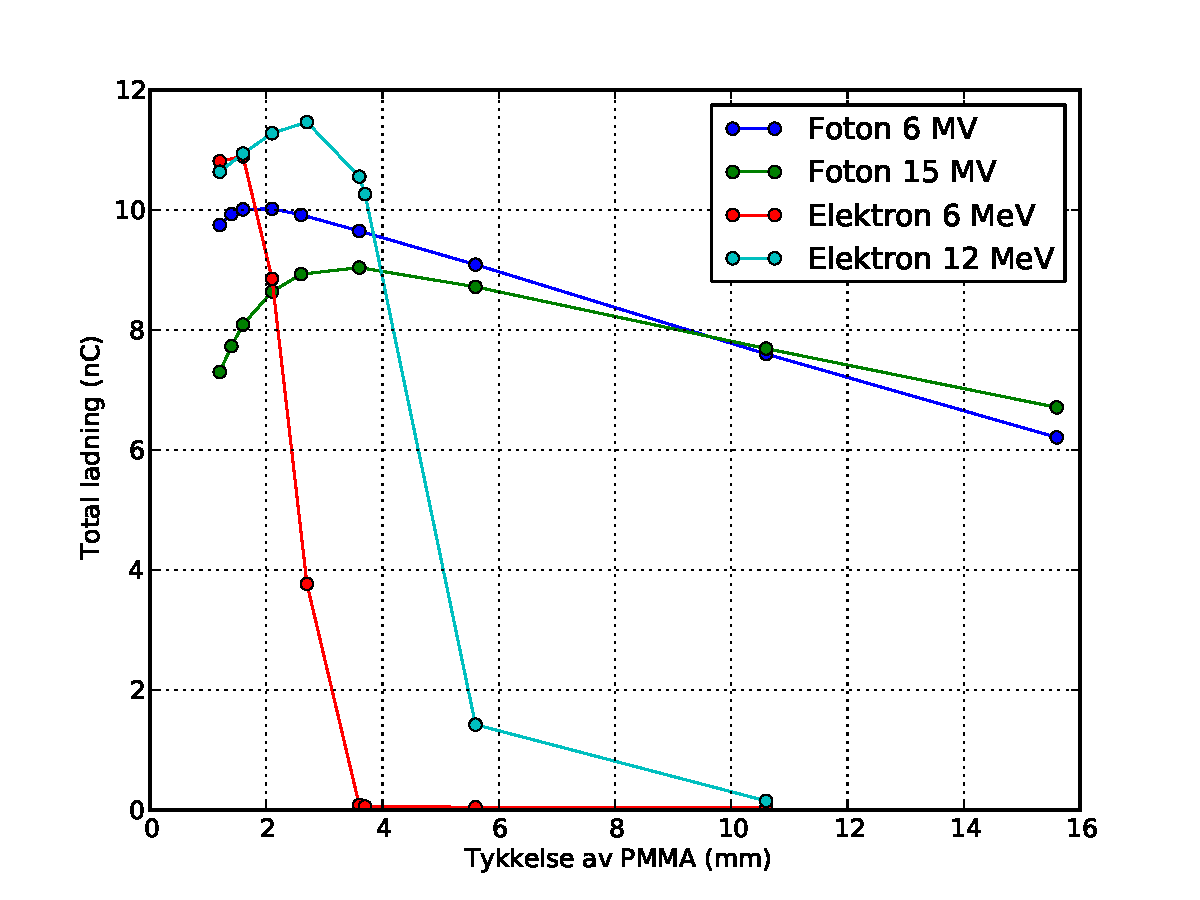
\includegraphics[width=\textwidth]{dybdedose}
 \caption{Målte dybdedosekurver for bestråling med fotoner og elektroner.}
\end{figure}

Fotonkurvene når sitt maksimum et lite stykke inn i mediet, dette skyldes build-up effekter foresaket av sekundærelektroner. Vi ser at de mest energirike fotonene har sin topp litt lenger inn i mediet. Samtidig ser vi at de mer energirike fotonene har en slakere decay innover i mediet, og at denne decayen ser tilnærmet lineær. Vi vet at energiavsetning fra fotoner i et medie skjer gjennom tre prosesser: fotoelektrisk effekt, comptonspredning og pardannelse.

For elektronene ser vi at de har en topp veldig kort inn i mediet, og faller så meget sterkt av, mye raskere enn fotonene. Igjen ser vi at elektronene med høyere energi har sin topp litt lenger inn i mediet. Elektronstråling er ladd-partikkelstråling og beskrives dermed av Bethe-Bloch.

\subsection{Tverrscan}
Vi plotter de målte verdiene og får plottet vist i figur 4.
\begin{figure}[htpb]
\centering
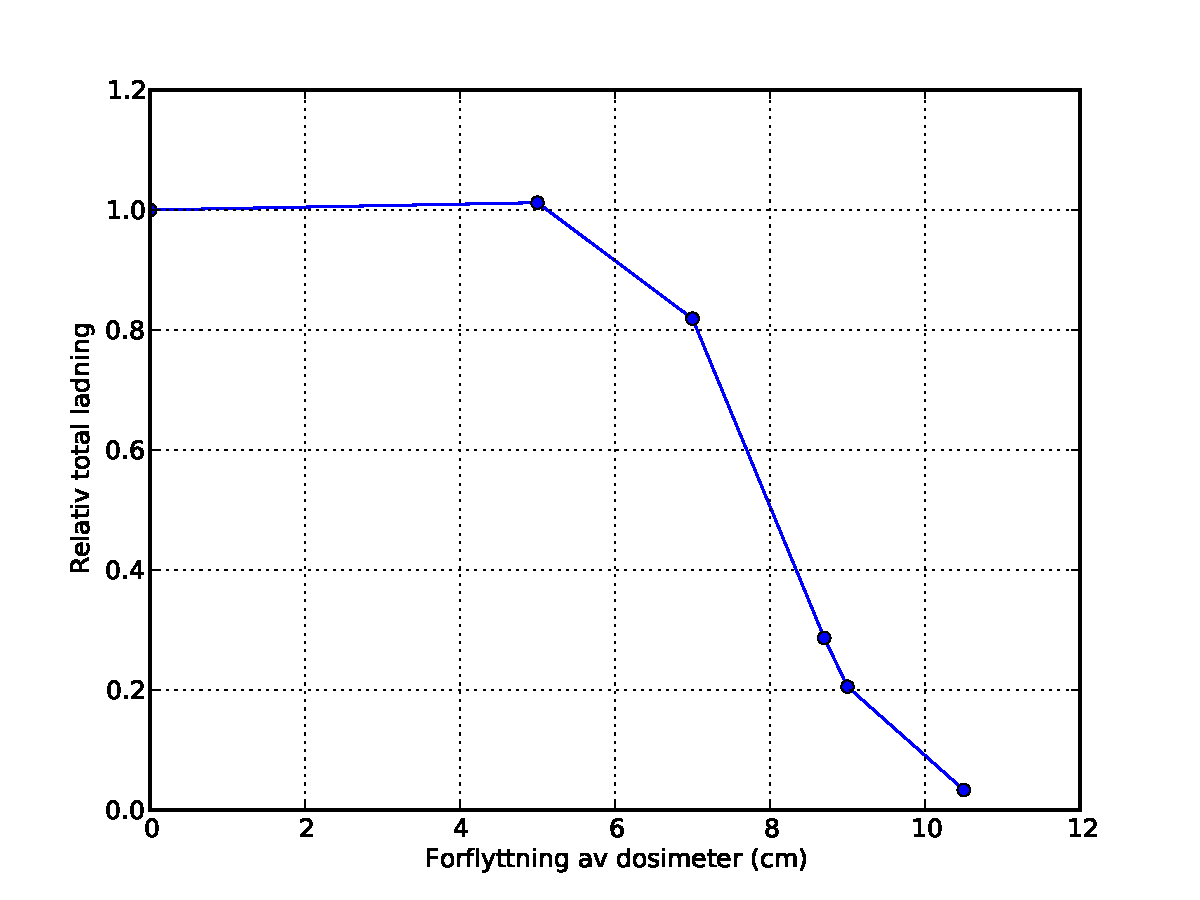
\includegraphics[width=\textwidth]{tverrscan}
\caption{Målinger ved tverrscan av elektronfelt.}
\end{figure}

Vi ser at de målte dosene holder seg relativt konstant en god stund. Dette er fordi dosimeteret starter midt i det kvadratiske 17.5 x 17.5 cm elektronfeltet, og det faller ikke noe særlig av før det begynner å nærme seg kanten. Feltet er definert slik at det skal ha halv verdi av midtverdi på kanten, i vårt tilfelle svarer kanten til en forflyttning på 8.75 cm fra sentrum, og der ser vi at den relative amplituden er ca 0.3, altså ikke akkurat halvparten, men ganske nærme.

\section{Konklusjon}
Vi har sett fra dybdedosekurven at både fotonstråling og elektronstråling vil ha en topp litt innover i mediet på grunn av build-up effekter (sekundærelektroner). I begge tilfeller ser vi at toppen vil havne lenger innover i mediet for større partikkelenergier. Vi ser også at elektronstrålingen faller så mye raskere mot null videre innover i vevet, mens fotonstrålingen er relativt sett mye mer slakt. For fotonene ser vi en klar tendens til at høyereenergifotoner har en slakere decay innover i mediet.

Fra tverrscannet har vi sett at feltet som produseres av lineærakseleratoren ikke faller veldig skarpt nær kanten, men har en mer gradvis decay utover. Feltets kant er definert som der feltet skal ha falt til halvparten, men vi målte at den hadde falt til en tredel.






\end{document}
